%% Based on a TeXnicCenter-Template by Tino Weinkauf.
%%%%%%%%%%%%%%%%%%%%%%%%%%%%%%%%%%%%%%%%%%%%%%%%%%%%%%%%%%%%%

%%%%%%%%%%%%%%%%%%%%%%%%%%%%%%%%%%%%%%%%%%%%%%%%%%%%%%%%%%%%%
%% HEADER
%%%%%%%%%%%%%%%%%%%%%%%%%%%%%%%%%%%%%%%%%%%%%%%%%%%%%%%%%%%%%

\documentclass[a4paper,onesided,10pt]{article}


%% Language %%%%%%%%%%%%%%%%%%%%%%%%%%%%%%%%%%%%%%%%%%%%%%%%%
\usepackage[USenglish]{babel} %francais, polish, spanish, ...
\usepackage[T1]{fontenc}
\usepackage[ansinew]{inputenc}

\usepackage{lmodern} %Type1-font for non-english texts and characters


%% Packages for Graphics & Figures %%%%%%%%%%%%%%%%%%%%%%%%%%
\usepackage{graphicx} %%For loading graphic files
%\usepackage{subfig} %%Subfigures inside a figure
%\usepackage{pst-all} %%PSTricks - not useable with pdfLaTeX


%% Math Packages %%%%%%%%%%%%%%%%%%%%%%%%%%%%%%%%%%%%%%%%%%%%
\usepackage{amsmath}
\usepackage{amsthm}
\usepackage{amsfonts}


\usepackage{fancyhdr} 
\pagestyle{fancy}
\fancyhf{}
\rhead{\small\leftmark}
\lhead{Jochen K. Illerhaus}
\rfoot{\thepage}

%Double spacing, just for the wirghting senter
%\openup 1em


%%%%%%%%%%%%%%%%%%%%%%%%%%%%%%%%%%%%%%%%%%%%%%%%%%%%%%%%%%%%%
%% DOCUMENT
%%%%%%%%%%%%%%%%%%%%%%%%%%%%%%%%%%%%%%%%%%%%%%%%%%%%%%%%%%%%%
\begin{document}

\pagestyle{empty} %No headings for the first 

\begin{titlepage}

\begin{center}

%\vspace*{1cm}
\Large
\textsc{Planet Simulator}\\

\vspace{5cm}

%\LARGE
\textsc{Honors Project\\[0.5\baselineskip]
by\\[0.5\baselineskip]
Jochen K. Illerhaus}

\vspace{5cm}
\textsc{\today}\\ %%Date - better you write it yourself.

\vspace{1cm}
\textsc{Supervisor:\\
Dr. Wojciech L. Golik}\\

\vspace{1cm}
\textsc{St. Charles (MO) Linendenwood University\\
School of Science\\
Institute of Mathematics}\\

\end{center}

\end{titlepage}

\tableofcontents 

\newpage

\pagestyle{fancy} 


%%%%%%%%%%%%%%%%%%%%%%%%%%%%%%%%%%%%%%%%%%%%%%%%%%%%%%%
\section{Abstract}
\textbf{TODO: WRITE THE ABSTRACT!!!}

%%%%%%%%%%%%%%%%%%%%%%%%%%%%%%%%%%%%%%%%%%%%%%%%%%%%%%%
\section{Introduction}

\subsection{Problem}
The task was to write some software that would visualize the motion of bodies (planets) in a gravitational system (Solar System). The simulation was to show the motion of those bodies from the perspective of one one of them. This would than show the Apparent Retrograde Motions \footnote{Apparent Retrograde Motion is the phenomenon of planets appearing to move backward when observed form another planets} of planets.

\subsection{Personal Motivation}
Computers have always fascinated me. Hence I enjoyed the chance to write a complicated and interesting peace of software. It was in the nature of the problem that I would have to work with computer graphics which is a part of computer programming that I particularly enjoy because I like seeing things move on my screen. I also have the dream to one day, write a computer game. This solar system project would allow me to work with some things important to fulfill that dream.

\subsection{Prior Knowledge}
I started to write my first programs four years ago initially using C++. Since than, I have been constantly improving my knowledge of computer programming and computer science although I never took any organized classes on computer programming. At the starting point of the project I was confident with C++, Java, Python, JavaScript, and Scilab (a clone of Matlab). I had done some data visualization and I had written some simple games. For their graphical parts, I had used the libraries: Swing (generic Java), Standard Windows API (C++), OpenGL through Glew (in both C++ and Java), Matplotlib (Python Anaconda), and I had worked with the direct manipulation of pixel data (in C++, Java, Python, and JavaScript). I had had three years of Physics in high school (3 semesters of them were calculus based) and I was rewarded with a membership in the German Society of Physicist for academic excellency in that subject. Those classes gave me a fundamental understanding of Newtonian Physics and Newtonian Gravity.


%%%%%%%%%%%%%%%%%%%%%%%%%%%%%%%%%%%%%%%%%%%%%%%%%%%%%%%
\section{Programming Language}

\subsection{Selection of the Programming Language}
I planed to select a programming language that I was already familiar with. On top of this, I wanted to write a "`big"' application,  not just a simple visualization. Further more a I anticipated that the result would have to be runnable without unusual external dependencies (that was a knockout for programs like Mathematica or Matlab). It would have been impractical to learn a new language just for this project. So, I had to choose form Python, Java and C++. Which one I picked didn't really matter, and I selected C++ for no particular reason.

\subsection{Selection of the Graphics Library}
I picked OpenGL (glew) as my graphics library knowing that this was not the easiest method to create graphics. There are many libraries, e.g. Matplotlib (for Python), available that offer easy tools that allow the creation of a simple plots in only a few lines. OpenGL on the other hand is a massive graphics library. The libraries API is as close to the hardware as it will get. When implemented correctly, OpenGL usually offers the best performance possible. OpenGL is commonly used for video games, computer aided design, movies, etc. This makes it an very important tool, hence the knowledge of its API is a valuable skill. So the main reason for selecting OpenGL was that I wanted to get familiar with it's API. As mentioned, I had worked with OpenGL befor but I had always used OpenGL 1.0 which does not use features like a programmable rendering pipeline or the exclusive use of buffer objects. I was looking forward to learn a new OpenGL based techniques. OpenGL requires the use of linear algebra to calculate transformations \footnote{It is also possible to use a mathematically much cleaner approach through Quaternions $\mathbb{H}$ }, manipulate positions, etc. In C++ the library OpenGL Mathematics (GLM) is often used for those tasks so I used it for this project as well.


%%%%%%%%%%%%%%%%%%%%%%%%%%%%%%%%%%%%%%%%%%%%%%%%%%%%%%%
\section{Planet Motion}
Obtaining the Planets positions as time progresses is obviously a key requirement. There are two options to do so that presents themselves. Firstly, planets move on conic sections that can be described in symbolic equations. A planets position at an arbitrary point in time may than be found by evaluating those symbolic expression. Second, some numerical method can be used solve a system of differential equations that describes the motion of those planets. Those differential equations would follow directly form a mathematical description of gravity (either Newton or Special Relativity). Given that my first idea would only involve evaluating some equations I was sure that this would be the easiest way but I was also curious to see whether or not my second thought would work the way I expected it to. Approximating the solution to a differential equation would also have the advantage that it would be a real simulation. Additionally to fulfilling the requirements of this task this would also allow answering questions like: What would happen if a gigantic comet crashed into Mars and slowed it down considerably? In the end I used both methods. I first wrote a solver (using Forward Euler Method) for the differential equation that follows form Newtons law of gravity and than implemented my first idea by reading in orbital elements and calculating the planets positions form them.

\subsection{Planet Motion as Solutions of Differential Equations}
Gravity was first described by Newton through the equation:
\begin{equation}
\vec{F_G} = \gamma \frac{mM}{r^2}\hat{r}
\label{eq:NewtonGravi}
\end{equation}
Where $\vec{F_G}$ is the Gravitational force that body $A$ exerts on body $B$, $\gamma$ is the Gravitaionla Konstant ($\gamma \approx  6.67 10^{-11} m^3 kg^{-1} s^{-2}$), $m$ is the mass of $B$, $M$ is the mass of $A$, $r$ is the distance between the centers of mass of $A$ and $B$, and $\hat{r}$ is a unit vector pointing form the center of mass of $B$ to the center of mass of $A$.
A fundamental part of Newtons mechanics is Newtons Second Law:
\begin{equation}
\vec{F} = m \ddot{\vec{x}}
\label{eq:NewtonsSecond}
\end{equation}
Where $\vec{F}$ is the Force, $m$ the mass and $\ddot{\vec{x}}$ the second derivative with respect to time of the position.

Form equations \ref{eq:NewtonGravi} and \ref{eq:NewtonsSecond} follows that:
\begin{equation}
\ddot{\vec{x}} = \gamma \frac{M}{r^2} \hat{r}
\label{eq:diffEqOne}
\end{equation}
This differential equation relates the second derivative of the position of body $B$ to its position (hidden in the corresponding $r$and $\hat{r}$). It is of second order and non linear. To reduce this to a first order problem that can be solved with standardized methods, the substitution $\vec{v} = \dot{\vec{x}}$ can be used. This reduces the problem to a system of non linear first order differential equations:
\begin{equation}
\left\{ \begin{tabular}{l}
$\dot{\vec{v}} = \gamma \frac{M}{r^2} \hat{r}$ \\
$\dot{\vec{x}} = \vec{v}$
\end{tabular}\right.
\label{eq:FirstSystem}
\end{equation}
The problem with \ref{eq:FirstSystem} is that it only considers a system of two bodies. In practice it is often possible to ignore the influence of most gravitational bodies except for one central body. For example, a model of the solar system can reach a reasonable degree of precession without considering the gravitational influence that the planets have on each other. Once this approximation is accepted, each planet could be considered as a individual two body problem (sun and planet). But I wanted to go through a more accurate model that would allow the simulation of binary stars and other special cases that require the consideration of the gravitational influences of all bodies in the system. Since in those cases \ref{eq:FirstSystem} has to hold pairwise for all bodies in the system it is a reasonable approach to simply sum all gravitational forces exerted on a given planet and than use the resulting force in a system of differential equations similar to \ref{eq:FirstSystem}. The resulting system of differential equations, that describes the motion of body $A$ is:
\begin{equation}
\left\{ \begin{tabular}{l}
$\dot{\vec{v}} = \gamma \sum_{i \in I}{\frac{M_i}{r_i^2} \hat{r_i}}$ \\
$\dot{\vec{x}} = \vec{v}$
\end{tabular}\right.
\label{eq:SecondSystem}
\end{equation}
Where $I$ is the set of all bodies except $A$, $M_i$ is the mass of body $i$, $r_i$ is the distance from the center of mass of body $A$ to the center of mass of body $i$, and $\hat{r_i}$ a unit vector pointing in the direction of that distance.

The delima with this system of differential equations is that the future positions can only be found if the future forces are known and the future forces can only be found if the future positions are known. My solution was to define a small time step $\Delta t$ and assume that the gravitational forces would not change during that time step. In reality, the gravitational Forces change continuously but it turns out that a small $\Delta t$ is close enough to obtain reasonably accurate results. With the definition of $\Delta t$ time can be considered as an integer $n$ such that $t = n \Delta t$. It follows form \ref{eq:SecondSystem} that:
\begin{equation}
\vec{a_n} = \gamma \sum_{i \in I}{\frac{M_i}{r_i^2}} \hat{r_i}  
\hspace{4mm} ; \hspace{4mm}  
\vec{v_{n+1}} = \vec{a_n} (1+\Delta t)   
\hspace{4mm} ; \hspace{4mm}  
\vec{x_{n+1}} = \vec{v_n} (1+\Delta t)
\label{eq:ForwardEuler}
\end{equation}
Using \ref{eq:ForwardEuler}, the planets positions can be obtained through iterating over $n$. Initial conditions ($\vec{v_0}$ and $\vec{x_0}$) have to be known and are input parameters.

\textbf{Note} This method is called \textit{Forward Euler} and its error grows linearly with $\Delta t$ \cite{NSDE}. Forward Euler is vary bad numerical method for the approximation of periodic solutions there are more advances methods \cite{NSDE} but Forward Euler is simple enough that I could develop the method myself and if a small enough $\Delta t$ is picked the results are still reasonably accurate.

As Figure \ref{fig:presection} shows, the choice of $\Delta t$ influences both the precision of the approximation. I picked a very small $\Delta t$ (exactly how small, is a parameter that is read in together with the other input data) \footnote{A small $\Delta t$ also goes with a high computational cost}.

\begin{figure}[h!]
	\centering
		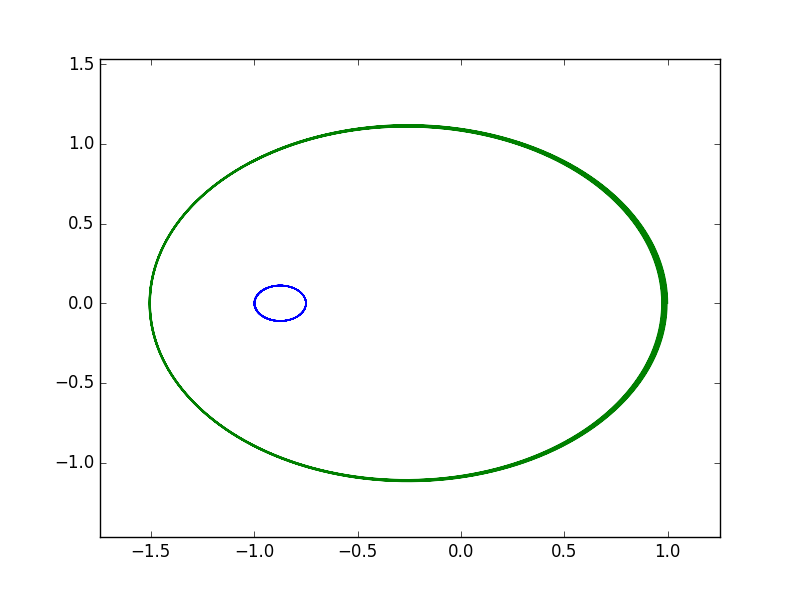
\includegraphics[width=0.45\textwidth]{2_Planets_0-001.png}
		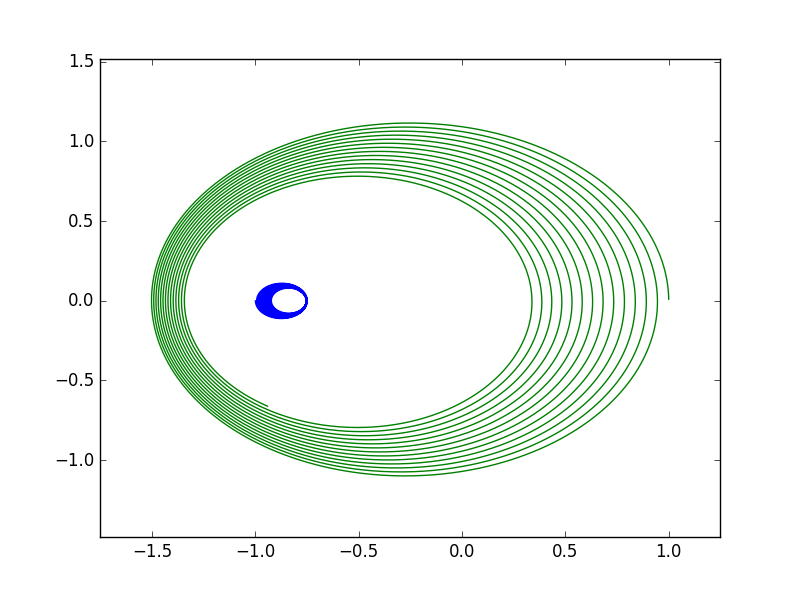
\includegraphics[width=0.45\textwidth]{2_Planets_0-02.png}
	\caption{\textit{Left:} The Orbits of two planets with $\Delta t = 0.001$ and 100000 steps \hspace{\textwidth}
		\textit{Right:} The Orbits of two planets with $\Delta t = 0.02$ and 5000 steps \hspace{\textwidth}
		Both use the same initial conditions}
	\label{fig:presection}
\end{figure}
\begin{figure}[h!]
	\centering
		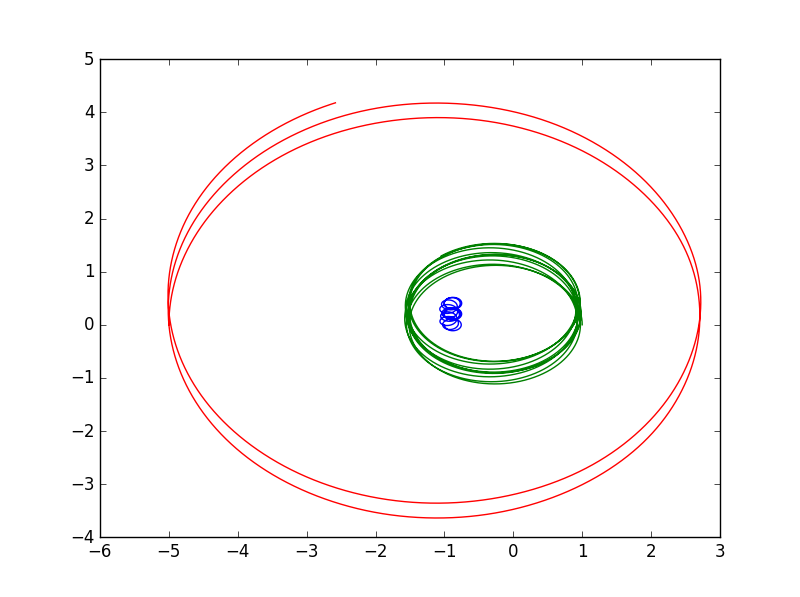
\includegraphics[width=0.45\textwidth]{3_Planets_0-001.png}
	\caption{Orbits of 3 planets in the system ($\Delta t = 0.001$)}
	\label{fig:3_Planets_0-001}
\end{figure}

\subsubsection{Assumptions and Simplifications}
The latest models for planetary motions take many effects into account. As described above I am only considering Newtonian Gravity. This leaves out many effects (especially General and Special Relativity). But since the numerical method used goes with a very high error, considering any of those effects does not appear to be helpful.


\subsection{Planetary Motion Derived from Kepler Elements}
Another idea was to consider the orbits of those bodies as conic sections. Because the visualization was only interested in planets the only important type of conic section would be the ellipse.

In the easiest case, planetary motion on elliptical orbits can be described in polar coordinates using the eccentricity ($e$) and length of the semi-major axis ($a$) of the Ellipse as parameters. The state vector ($\vec{s} = \left\langle\begin{array}{c}r, \Theta, v, \omega \end{array}\right\rangle$) can than be described as a function of time an converted to Cartesian coordinates. The result can than expresses the state of the body on a plain in $\mathbb{R}^3$ were the position and velocity are each element of $\mathbb{R}^2$ to rewrite the coordinates of the planet on the plain in terms of the global base, a simple matrix transformation can be applied to the position and velocity of the planet. This is a common concept (see  \cite{KOECSV} \cite{KEAP}).


%%%%%%%%%%%%%%%%%%%%%%%%%%%%%%%%%%%%%%%%%%%%%%%%%%%%%%%
\section{Apparent Retrograde Motion}
The main task of the project was visualizing the apparent retrograde motion of planets as seen form other planets. The effect is a consequence of planets having different orbital periods. Since the Gravitational force acts as a centripetal force (assuming circular orbits), the planets will have different tangential velocities, and path lengths, hence their years will be of different lengths:
\begin{equation}
F_G = F_c \Leftrightarrow 
\gamma \frac{mM}{r^2} = m {\left( \frac{2 \pi r}{ T } \right)}^2 \frac{1}{r} \Rightarrow 
T = \sqrt{ \frac{4 \pi^2}{\gamma M} r^3 } \Rightarrow 
T \propto r^{ {}^3 / {}_2 }
\label{eq:TangentialVelocities}
\end{equation}

\begin{figure}[h!]
	\centering
		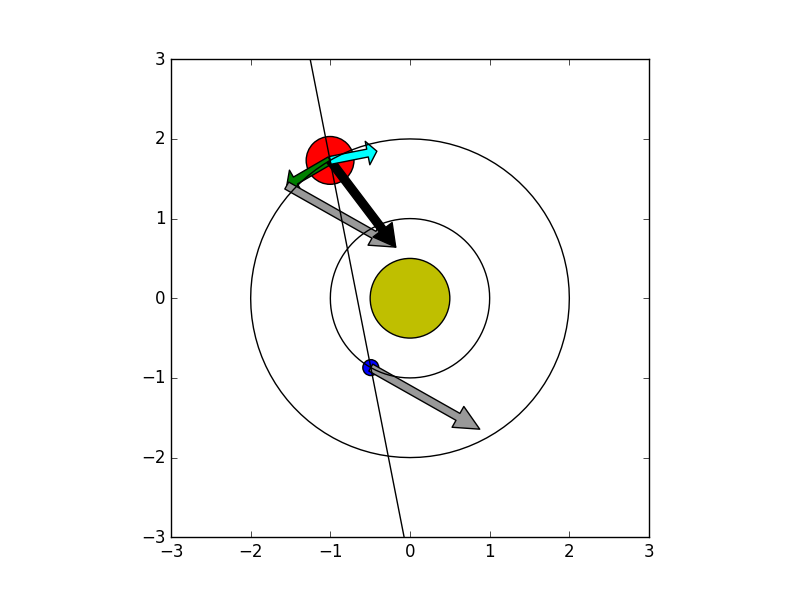
\includegraphics[width=0.80\textwidth]{overview.png}
	\caption{The velocities as seen form earth: gray: $\vec{v}$, green: $\vec{u}$, black: $\vec{v}+\vec{u}$, blue: $\vec{w}$}
	\label{fig:overview}
\end{figure}

This is not the velocity observed form Earth, but from the center of Gravity of the system. A observer on a planet will move together with that planet. In the best case this would allow the observer to see the sum of his/her own velocity vector $\vec{v}$ and the velocity of the observed planet $\vec{u}$. A second effect is caused because any observer at a single point can only observe a 2D projection of the 3D universe. Visible for the observer is only the projection vector $\vec{w}$ of the $\vec{v}+\vec{u}$ vector on a plain perpendicular to the connecting line form the observer to the observed object. Figure \ref{fig:overview} illustrates this in two dimensions. \textbf{Note:} Another type of the apparent retrograde motion of planets is caused by the planet rotating about its own axis. This effect is not considered in that project.

\begin{figure}[h!]
	\centering
		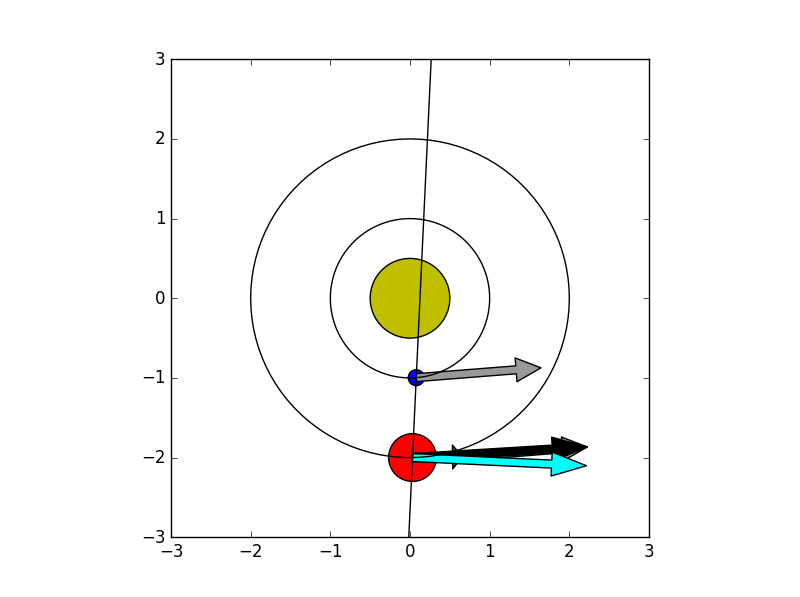
\includegraphics[width=0.45\textwidth]{adding.png}
		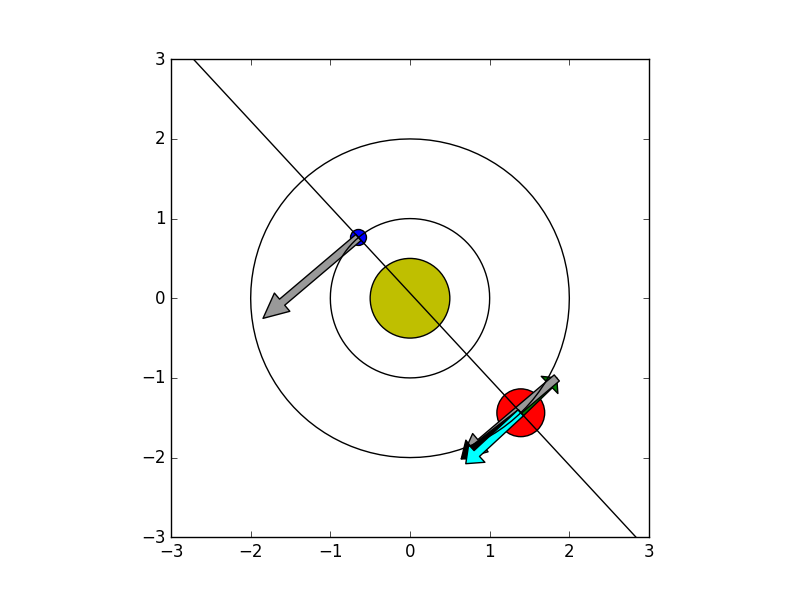
\includegraphics[width=0.45\textwidth]{subtracting.png}
	\caption{\textbf{Left:} the speed as observed from earth is at its positive extreme \hspace{\textwidth}
	\textbf{Right:} the speed as observed from earth is at its negative extreme}
	\label{fig:adding}
\end{figure}

Apparent retrograde motion occurs when $\vec{w}$ switches directions. Figure \ref{fig:adding} shows to extreme cases of apparent retrograde motion.


%%%%%%%%%%%%%%%%%%%%%%%%%%%%%%%%%%%%%%%%%%%%%%%%%%%%%%%
\section{User Manual}
The user interface (UI) of this program is bad. It heavily relies on third party software (to edit input files) and on key events. On top of that, neither the input files nor the keys follow a clear nor concise system. The user interface of this program could be greatly improved in a future project.

\subsection{General Operation}
The User Interface (UI) consists of an visual output and file, keyboard, and mouse inputs. The Output is split into two areas. The main area of the window shows an overview of the current scene. In the lower right hand corner, a separate panel shows the current scene as it could be observed from the center of the current planet. Whichever planet is currently selected, and some of its properties, is outputted as text in the upper left hand corner. An arrow in the upper right hand corner points towards the current planet's position. A bar chart on the right hand side informed about the energy that is currently in the planetary system. The yellow bar showed the total amount of energy (gravitational $+$ kinetic), the green bar represents the total kinetic energy of all bodies, and the red bar represents the total gravitational energy of all bodies. A body infinitely far away form all other bodies is considered to have a gravitational energy of $0$ and the coordinate system is defined to have a kinetic Energy of $0$. (Note: Each of these bars determines a reasonable scale on start up, those scales will not be equal).

\subsubsection{Camera}
The camera controls are inspired by the videogame Minecraft. Right-Mouse-Dragging allows to changing the Euler Angles of the direction the camera looks in. The camera position is set using the keyboard. The Keys $A$ and $D$ move the camera perpendicular to the projection of the view direction, $W$ and $S$ move the camera along the view direction, shift and spacebar move the camera up and down \footnote{this setup is usually controlled with the left hand where the baby finger is placed on shift, the ring finger on $A$, the middle finger alternates between $W$ and $S$, the index finger controls $D$ and the thumb is used for the space bar}.

\subsubsection{Observation Mode}
Visualizing the apparent retrograde motion of planets is done in Observation Mode. The Observation Mode is toggled on/off with the the $J$ key. In Observation Mode, the text on the left hand side expands and shows information about both: the current planet (at which the camera is stationed) and the observed planet (at which the camera is pointed). Observation Mode also shows the velocity vector of the observed planet projected such that it corresponds to the velocity as it would be perceived form earth. The length of this vector is also represented by a purple bar on the right hand side. The current planet can be changed with the TAB key (TAB jumps to the next planet TAB+B to the previous). The observed planet is change with CONTROL+TAB (CONTROL+TAB jumps to the next planet CONTROLE+TAB+B to the previous).

\subsubsection{Key-Map}
Here are all the functions of the keys:
\begin{itemize}
	\item \textbf{W, A, S, D, SHIFT, SPACE:} Move main camera forward, left, backward, right, down, up
	\itme \textbf{RIGHT\_MOUS\_BUTTON:} Slows down the speed at which W, A, S, D, SHIFT, SPACE move the camera trough space ("`sneaking"').
	\item \textbf{TAB, TAB+B:} Change the planet the on planet camera is on.
	\item \textbf{SHIFT+TAB, SHIFT+TAB+B:} Change the planet the on planet observes (observation mode only).
	\item \textbf{U:} Start/Stop simulation.
	\item \textbf{K:} Show coordinate system / stop showing it.
	\item \textbf{+, -:} Increase/decrease the speed of the simulation (Warning: Too high speeds can lead to performance and precision issues).
	\item \textbf{F5:} Reload the scene from the file. Can be used as "`Reset to initial conditions"'
	\item \textbf{F:} Move simulation forward by a single frame.
	\item \textbf{V:} Draw error symbolizing the velocities of the planets / stop drawing them.
	\item \textbf{J:} Enter/leave observation mode.
	\item \textbf{G:} Plot the gravitational force field as arrows / stop plotting it. Warning: A new scale for the arrows is determined every frame.
	\item \textbf{P:} Shows stationary randomly placed stars in the background / stops showing them.
	\item \textbf{T:} Draws 1000 data point long traces behind planets / stops drawing them.
	\item \textbf{PAGE\_UP, PAGE\_DOWN:} Increase/decrease the size of the on planet camera's display.
	\item \textbf{F2} Increase the size of the window.
	\item \textbf{ESC} Leave the program
\end{itemize}

\subsection{Input Files}
The initial conditions and parameters are read from an input file. A file picker would be a useful improvement but currently a fill called "`inputPlanetHorizen.txt"' in the working directory is loded. All input files are UTF-8 encoded text files and will usually use the extension '.txt'. The parsing of those files only catches view error and it is therefore essential that the input files are precisely correct. There are two fundamentally different protocols used which are distinguished by their first line: "`\#cartesian"' files specify the initial state vectors \footnote{If $\vec{x}$ is the position, $\vec{v}$ the velocity of a body than the state vector $\vec{s}$ is defined as $\vec{s} = \left\langle \vec{x}, \vec{v} \right\rangle$} in Cartesian coordinates, "`\#kepler"' files specify orbital elements of the orbits of those planets. Figures \ref{fig:inputPlanetHorizen} and \ref{fig:keplerModle} show examples for those input files both specifying the solar system. Because the program has problems determining the velocities of planets correctly when given orbital elements (through a "`\#kepler"' file), the use of those files is discouraged. In both file types, planets are assigned a name that has to consist of "`A-Z"', "`a-z"', "`0-9"', and/or "`\_"'. The files also allow three different scales for the planets radii. It is not practical to display e.g. the suns and the earths radius in proportion, hence it is possible to specify three scales "`Scale\_l"', "`Scale\_m"', and "`Scale\_s"'. In the coulomb size, each planet must specify which scale its radius is supposed to be multiplied by. This is done by entering one of the characters "`l"', "`m"', or "`s"'. The visualization also does some lighting calculations (but no shadows) and therefore needs information about which of the specified bodies will act as a light source. This is specified by either true or false in the "`isLight"' column \footnote{currently only one light source is supported, hence there is only one row can specify true in the "`isLight"' column}. The Visualization does not handle units, therefore it is up to the user to make the units of the input parameters match with each other and the gravitational constant provided. It is advisable to pick one unit for distances, one for time, and one for mass. Then all parameters can be expressed in terms of those units \footnote{Notice that none of the radii are relevant for the computations of position and velocity, hence may use a separate unit}. 

\begin{figure}
	\centering
		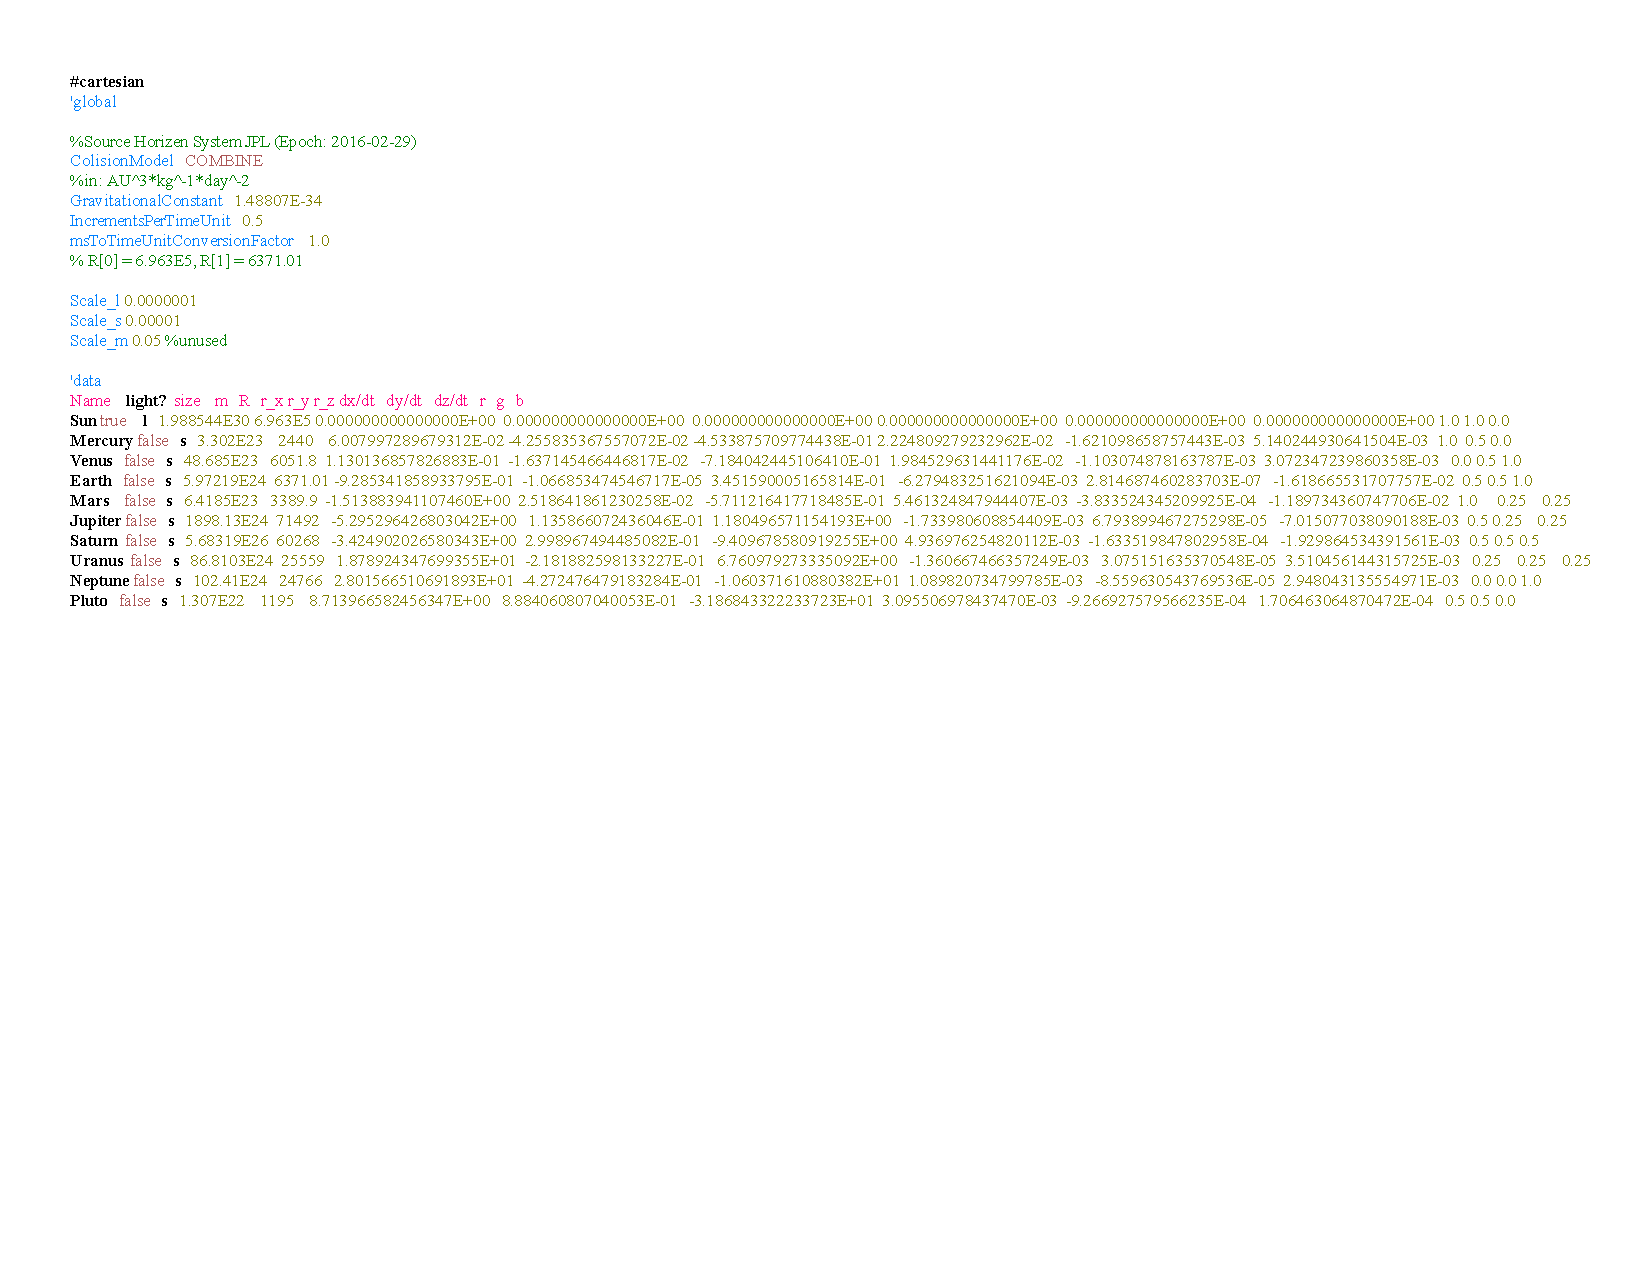
\includegraphics[width=1.6\textwidth, angle=90]{inputPlanetHorizen.pdf}
	\caption{Contents of an "`\#cartesian"' Input-File specifying the Cartesian state vectors of the Sun, Pluto and all major planets in the solar system}
	\label{fig:inputPlanetHorizen}
\end{figure}

\begin{figure}
	\centering
		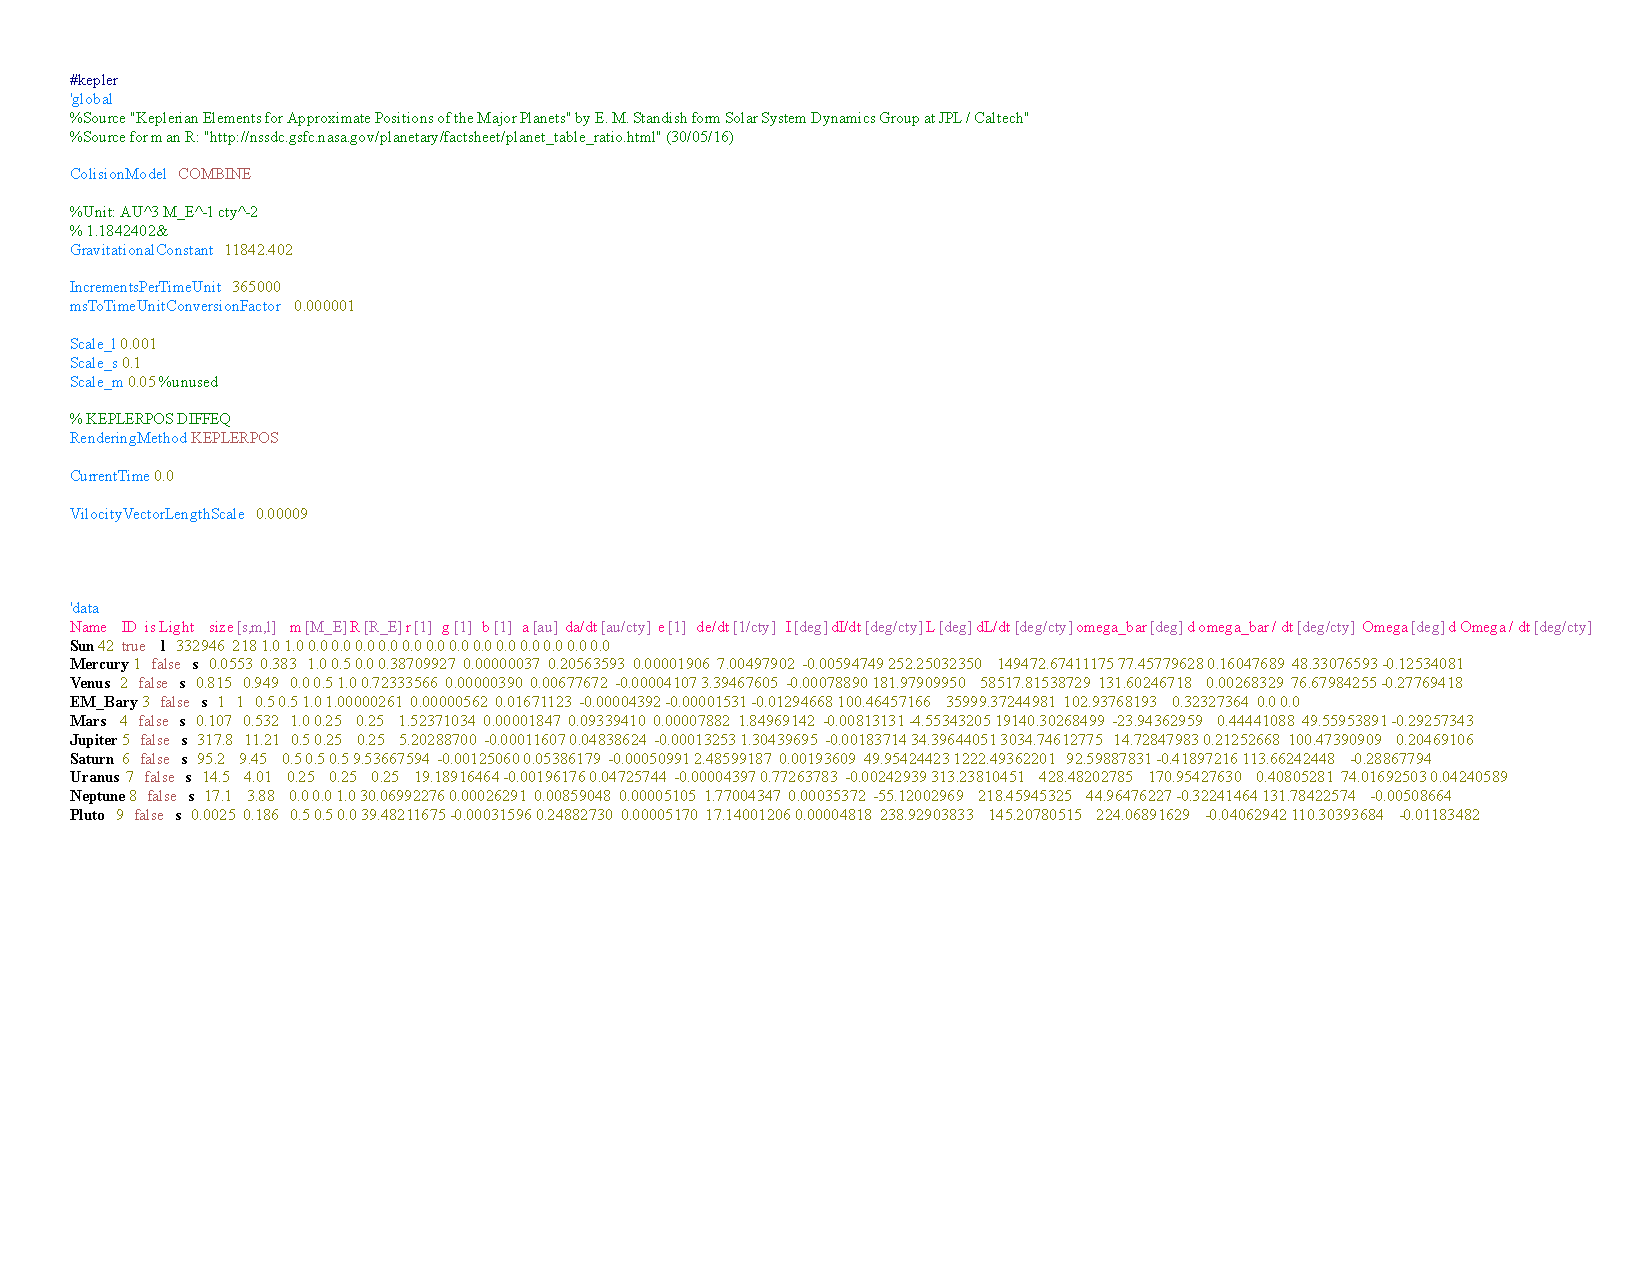
\includegraphics[width=1.6\textwidth, angle=90]{keplerModle.pdf}
	\caption{Contents of an "`\#kepler"' Input-File specifying the orbital elements of the Sun, Pluto and all major planets in the solar system}
	\label{fig:keplerModle}
\end{figure}


%%%%%%%%%%%%%%%%%%%%%%%%%%%%%%%%%%%%%%%%%%%%%%%%%%%%%%%
\section{Future Planes}
There are a lot of functions that I want to add into my visualizations:
\begin{itemize}
	\item Direct access to the Horizon System (JPL) to obtain orbital elements, state vectors and properties for various planets directly form JPL Solar System Mecanics .
	\item Improvements of the style of the the visualisation e.g through the use of texture, normal, and shadow maps or post processing effects.
	\item Change form the input files (from csv with a non standard header to some standard file system like xml or json)
	\item An actual graphical UI. Possibly using a mixture of OpenGL and Qt a graphical UI could massively improve user friendlessness.
	\item General improvements of the Key-Map. Especially reassigning the functions to new keys that are easier to remember.
	\item The main components of this program could be interfaced through Python and wrapped up in a python model to reduce development time without experiencing any major performance drawbacks.
	\item Optimizations of the rendering process, e.g. dynamically picking a reasonable vertex density would be helpful.
	\item Numerically finding the Lagrangian points of a given set of two planets.
	\item Sound Effects. Planetary motion is periodic just like sound. It might be possible to convert this motion into sound.
	\item Quaternions instead of linear algebra (a mathematically much nicer approach).
	\item Lagrangian Mechanics instead of Newtonian, could simplify the equations of motion.
\end{itemize}


%%%%%%%%%%%%%%%%%%%%%%%%%%%%%%%%%%%%%%%%%%%%%%%%%%%%%%%
\section{Lessons Learned}
I learned a lot during this project. I managed to widen my understanding of the following points:
\begin{itemize}
	\item 3D graphics using the Open Graphics Library (OpenGL): I learned OpenGL 3.0, which means that the programmable pipeline as well as most buffer objects were new to me.
	\item The programming language C++: I had written object oriented programs before but during this project I massively improved at applying the concept of object orientation. In particular at deciding when to split up functionality between different objects.
\end{itemize}
During the project I also learned some entirely new concepts:
\begin{itemize}
	\item Solving a differential equation numerical.
	\item Working continually on a supervised project. I had done projects of similar scale before, but I had usually not been supervised nor did I have a clear task to accomplish.
\end{itemize}


%%%%%%%%%%%%%%%%%%%%%%%%%%%%%%%%%%%%%%%%%%%%%%%%%%%%%%%
\clearpage
\section{Declaration of Originality}
I certify, as the author of this paper, that I was the
person primarily involved in the study designs, implementation, analysis and manuscript preparation. I
declare that the work presented in the paper is to the best of my knowledge and belief, original (except as acknowledged in the text).\\

\vspace*{15mm}

Jochen K. Illerhaus\\

%%%%%%%%%%%%%%%%%%%%%%%%%%%%%%%%%%%%%%%%%%%%%%%%%%%%%%%
\clearpage
\section{References}
\nocite{*} % to test all bib entrys
\bibliographystyle{unsrt}
\bibliography{PlaneteSimulatorDocumnetaion}
%\bibliographystyle{plain}

\appendix



\end{document}

